

% Gradient Info
  
\tikzset {_wou27m9t1/.code = {\pgfsetadditionalshadetransform{ \pgftransformshift{\pgfpoint{0 bp } { 0 bp }  }  \pgftransformrotate{-90 }  \pgftransformscale{2 }  }}}
\pgfdeclarehorizontalshading{_mx03xpnva}{150bp}{rgb(0bp)=(1,1,1);
rgb(37.5bp)=(1,1,1);
rgb(50.17857142857143bp)=(0,0,0);
rgb(62.5bp)=(1,1,1);
rgb(100bp)=(1,1,1)}
\tikzset{every picture/.style={line width=0.75pt}} %set default line width to 0.75pt        

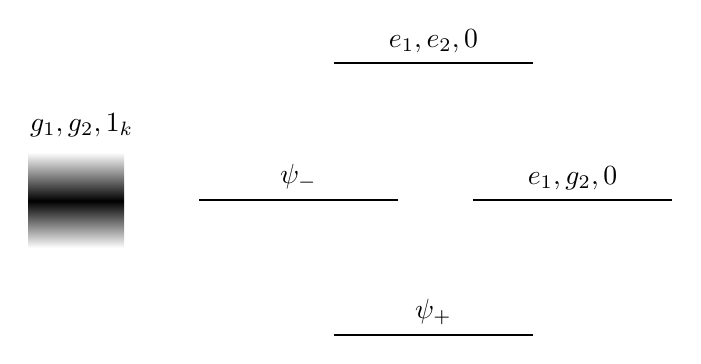
\begin{tikzpicture}[x=0.75pt,y=0.75pt,yscale=-1,xscale=1]
%uncomment if require: \path (0,300); %set diagram left start at 0, and has height of 300

%Straight Lines [id:da30984289381495134] 
\draw    (243,235) -- (339,235) ;
%Straight Lines [id:da9971381482409483] 
\draw    (243,104) -- (339,104) ;
%Straight Lines [id:da8148668338099976] 
\draw    (178,170) -- (274,170) ;
%Straight Lines [id:da11538291197175354] 
\draw    (310,170) -- (406,170) ;
%Shape: Square [id:dp6882035746519533] 
\draw  [draw opacity=0][shading=_mx03xpnva,_wou27m9t1] (96,147) -- (142,147) -- (142,193) -- (96,193) -- cycle ;

% Text Node
\draw (291,100.6) node [anchor=south] [inner sep=0.75pt]    {$\ket{e_{1} ,e_{2} ,0}$};
% Text Node
\draw (291,231.6) node [anchor=south] [inner sep=0.75pt]    {$\ket{\psi_+}$};
% Text Node
\draw (226,166.6) node [anchor=south] [inner sep=0.75pt]    {$\ket{\psi_-}$};
% Text Node
\draw (358,166.6) node [anchor=south] [inner sep=0.75pt]    {$\ket{e_{1} ,g_{2} ,0}$};
% Text Node
\draw (121.53,141.1) node [anchor=south] [inner sep=0.75pt]    {$\ket{g_{1} ,g_{2} ,1_{k}}$};


\end{tikzpicture}
